\documentclass{beamer}
\usetheme{Boadilla}

\beamertemplatenavigationsymbolsempty


\usepackage{beamer2pptx}


\title{Beamer2pptx}
\author{gion-xy}
\date{2018/2/12}

\begin{document}

\frame{\titlepage}

\begin{frame}{Add notes}
  First, you need to load \texttt{beamer2pptx.sty}: \\
  \texttt{\textbackslash usepackage\{beamer2pptx\}}

  Then you can insert notes with the following command: \\
  \texttt{\textbackslash pptxnotes\{Some comments\}}

  \pptxnotes{
    Comment
  }
\end{frame}


\begin{frame}{Overlay-specification-aware!}
  \texttt{\textbackslash pptxnotes} is overlay-specification-aware.

  \begin{itemize}[<+->]
  \item AAA
  \item BBB
  \end{itemize}

  \pptxnotes<1>{
    You can use non-ascii character in notes.
  }
  \pptxnotes<2>{
    非ASCII文字も使える.
  }
\end{frame}


\begin{frame}{Convert}
  \begin{itemize}
  \item \texttt{\% pip install python-pptx pdfminer.six}
  \item \texttt{\% python beamer2pptx.py} \textit{pdffile}
  \end{itemize}

  \begin{figure}
    \centering
    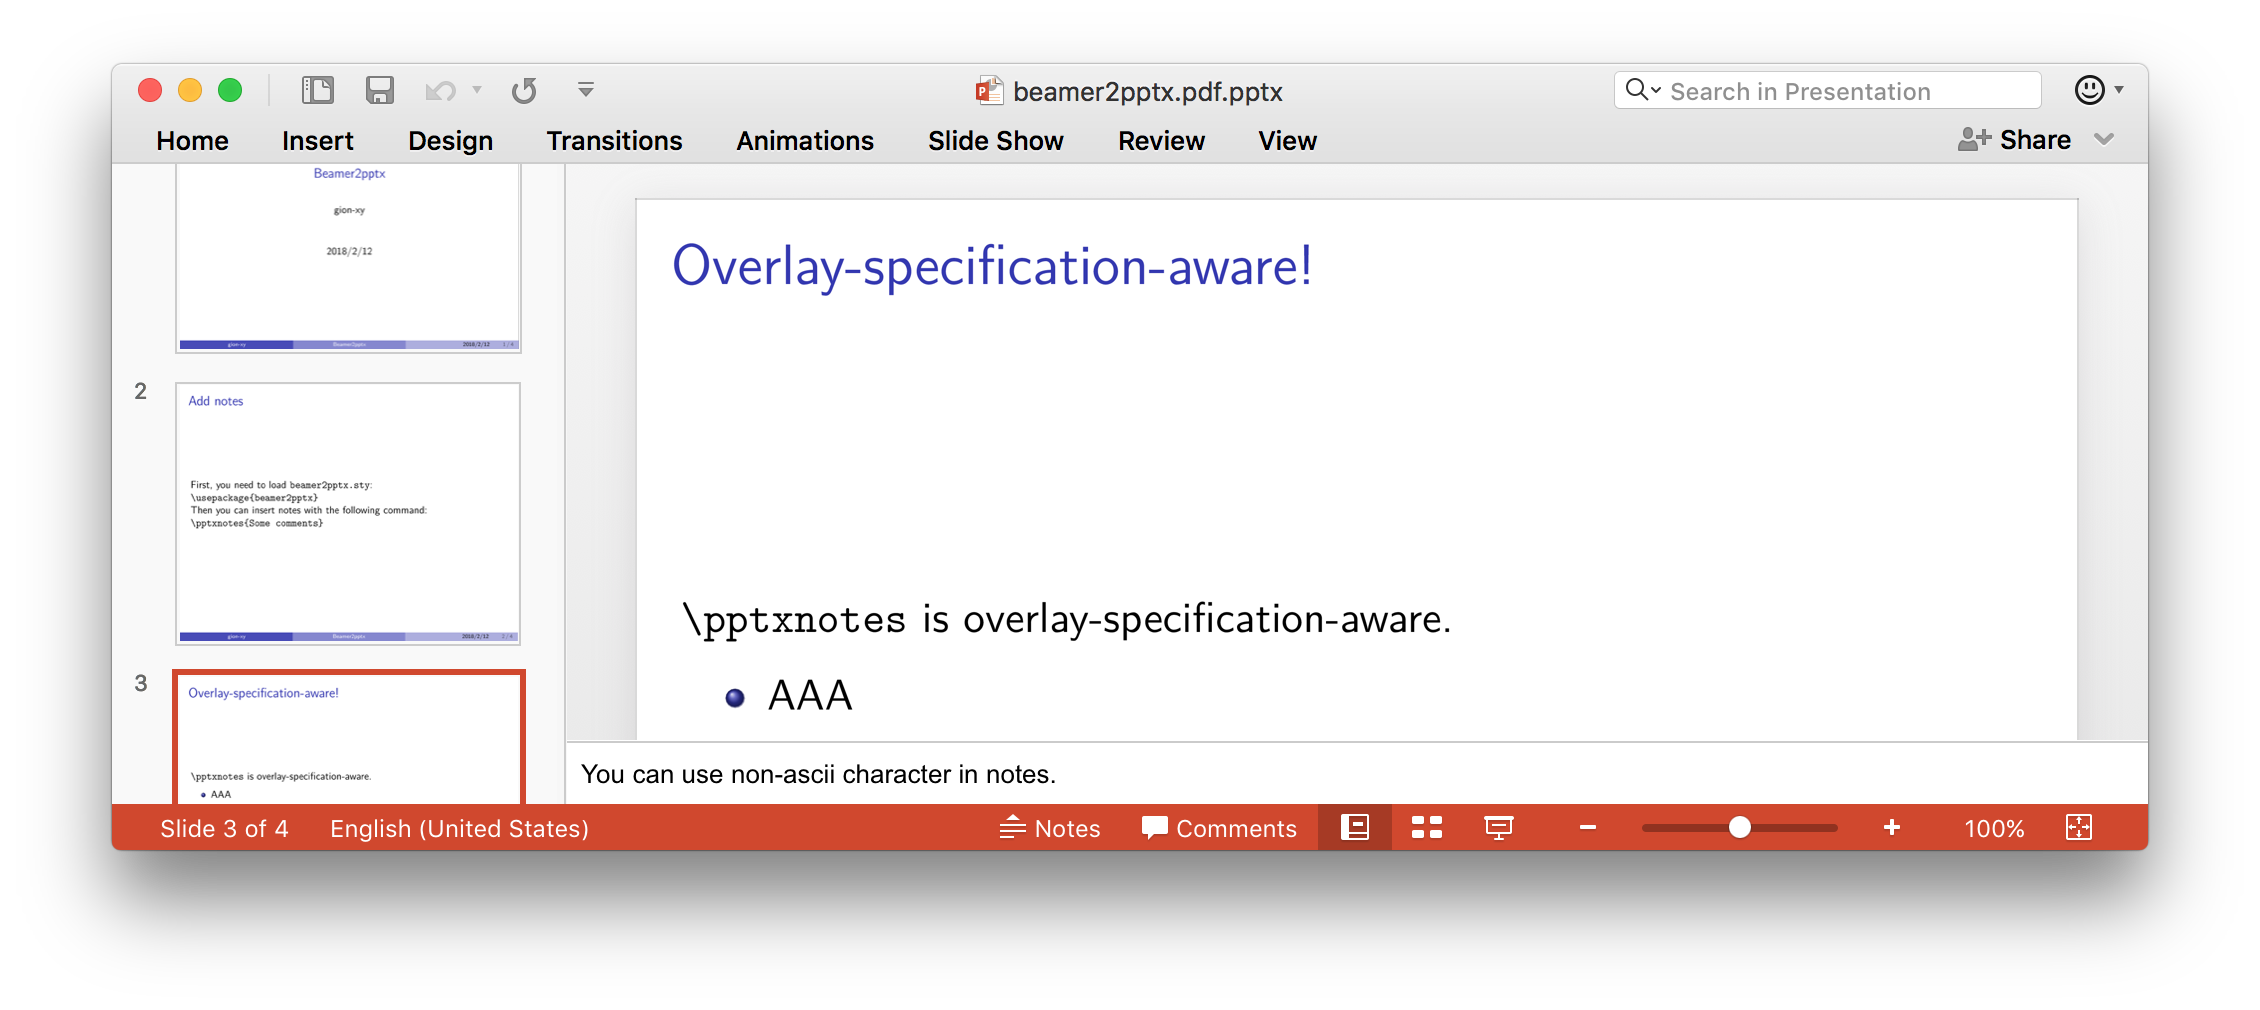
\includegraphics[width=\textwidth]{pptx-with-notes.png}
  \end{figure}
\end{frame}

\end{document}
